\section{Studia Przypadków}


\begin{columnframe}{Studium przypadku: Quest Carbon Capture and Storage Facility (Kanada)}
    \begin{column}{0.5\textwidth}
        \begin{figure}
            \centering
            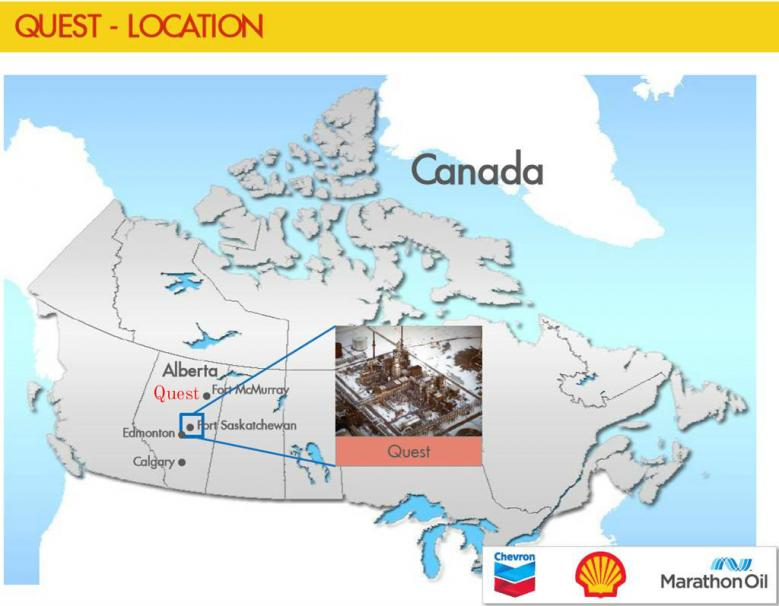
\includegraphics[width=0.6\textwidth, frame]{images/quest_alberta_canada_map.jpg}
        \end{figure}
    \end{column}
    \begin{column}{0.5\textwidth}
        \begin{itemize}
            \item Zbudowana w 2010 roku przez Shell Canada
            \item Wyłapuje CO$_2$ z wyniku produkcji wodoru (z metanu)
            \item 80km rurociągu
            \item do 3 Mt CO$_2$ rocznie
        \end{itemize}
    \end{column}
\end{columnframe}

\begin{frame}{Studium przypadku: Quest Carbon Capture and Storage Facility (Kanada)}
    \begin{figure}
        \centering
        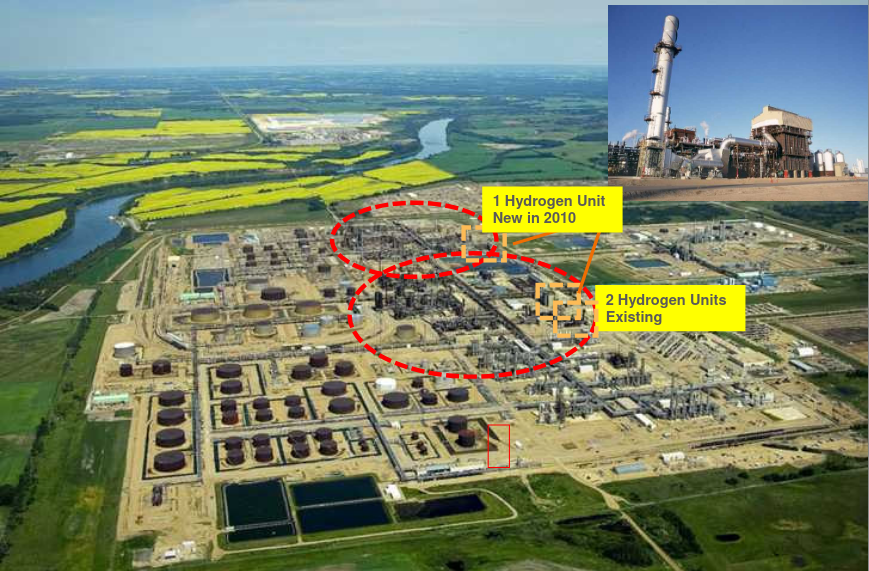
\includegraphics[width=0.9\textwidth, frame]{images/quest_ccs_hydrogen_farms.png}
    \end{figure}
\end{frame}

\begin{columnframe}{Petra Nova (Thompsons, Teksas, USA)}
    \begin{column}{0.5\textwidth}
        \begin{figure}
            \centering
            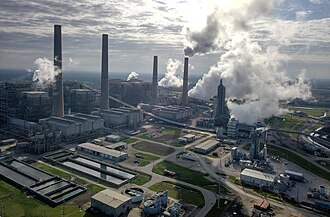
\includegraphics[width=0.9\textwidth, frame]{images/petra_nova_plant.jpg}
            \caption{Petra Nova (po prawej)}
        \end{figure}
    \end{column}
    \begin{column}{0.5\textwidth}
        \begin{itemize}
            \item Zbudowana w 2017 roku przez NRG Energy i JX Nippon Oil \& Gas Exploration
            \item 1.4 Mt CO$_2$ rocznie
            \item Wyłapuje ok. 30\% emisji CO$_2$ z sąsiadującej 240 MW-ej elektrowni węglowej
            \item CO$_2$ jest wykorzystywane do zwiększenia wydobycia ropy (EOR)
        \end{itemize}
    \end{column}
\end{columnframe}

\begin{columnframe}{Northern Lights (Øygarden, Norwegia)}
    \begin{column}{0.5\textwidth}
        \begin{itemize}
            \item 2600 metrów pod powierzchnią morza
            \item 1.5 Mt CO$_2$ rocznie, z możliwością zwiększenia do 5 Mt
            \item Pierwsza instalacja CCS w Norwegii, pierwsza międzynarodowa w Europie
        \end{itemize}
    \end{column}
    \begin{column}{0.5\textwidth}
        \begin{figure}
            \centering
            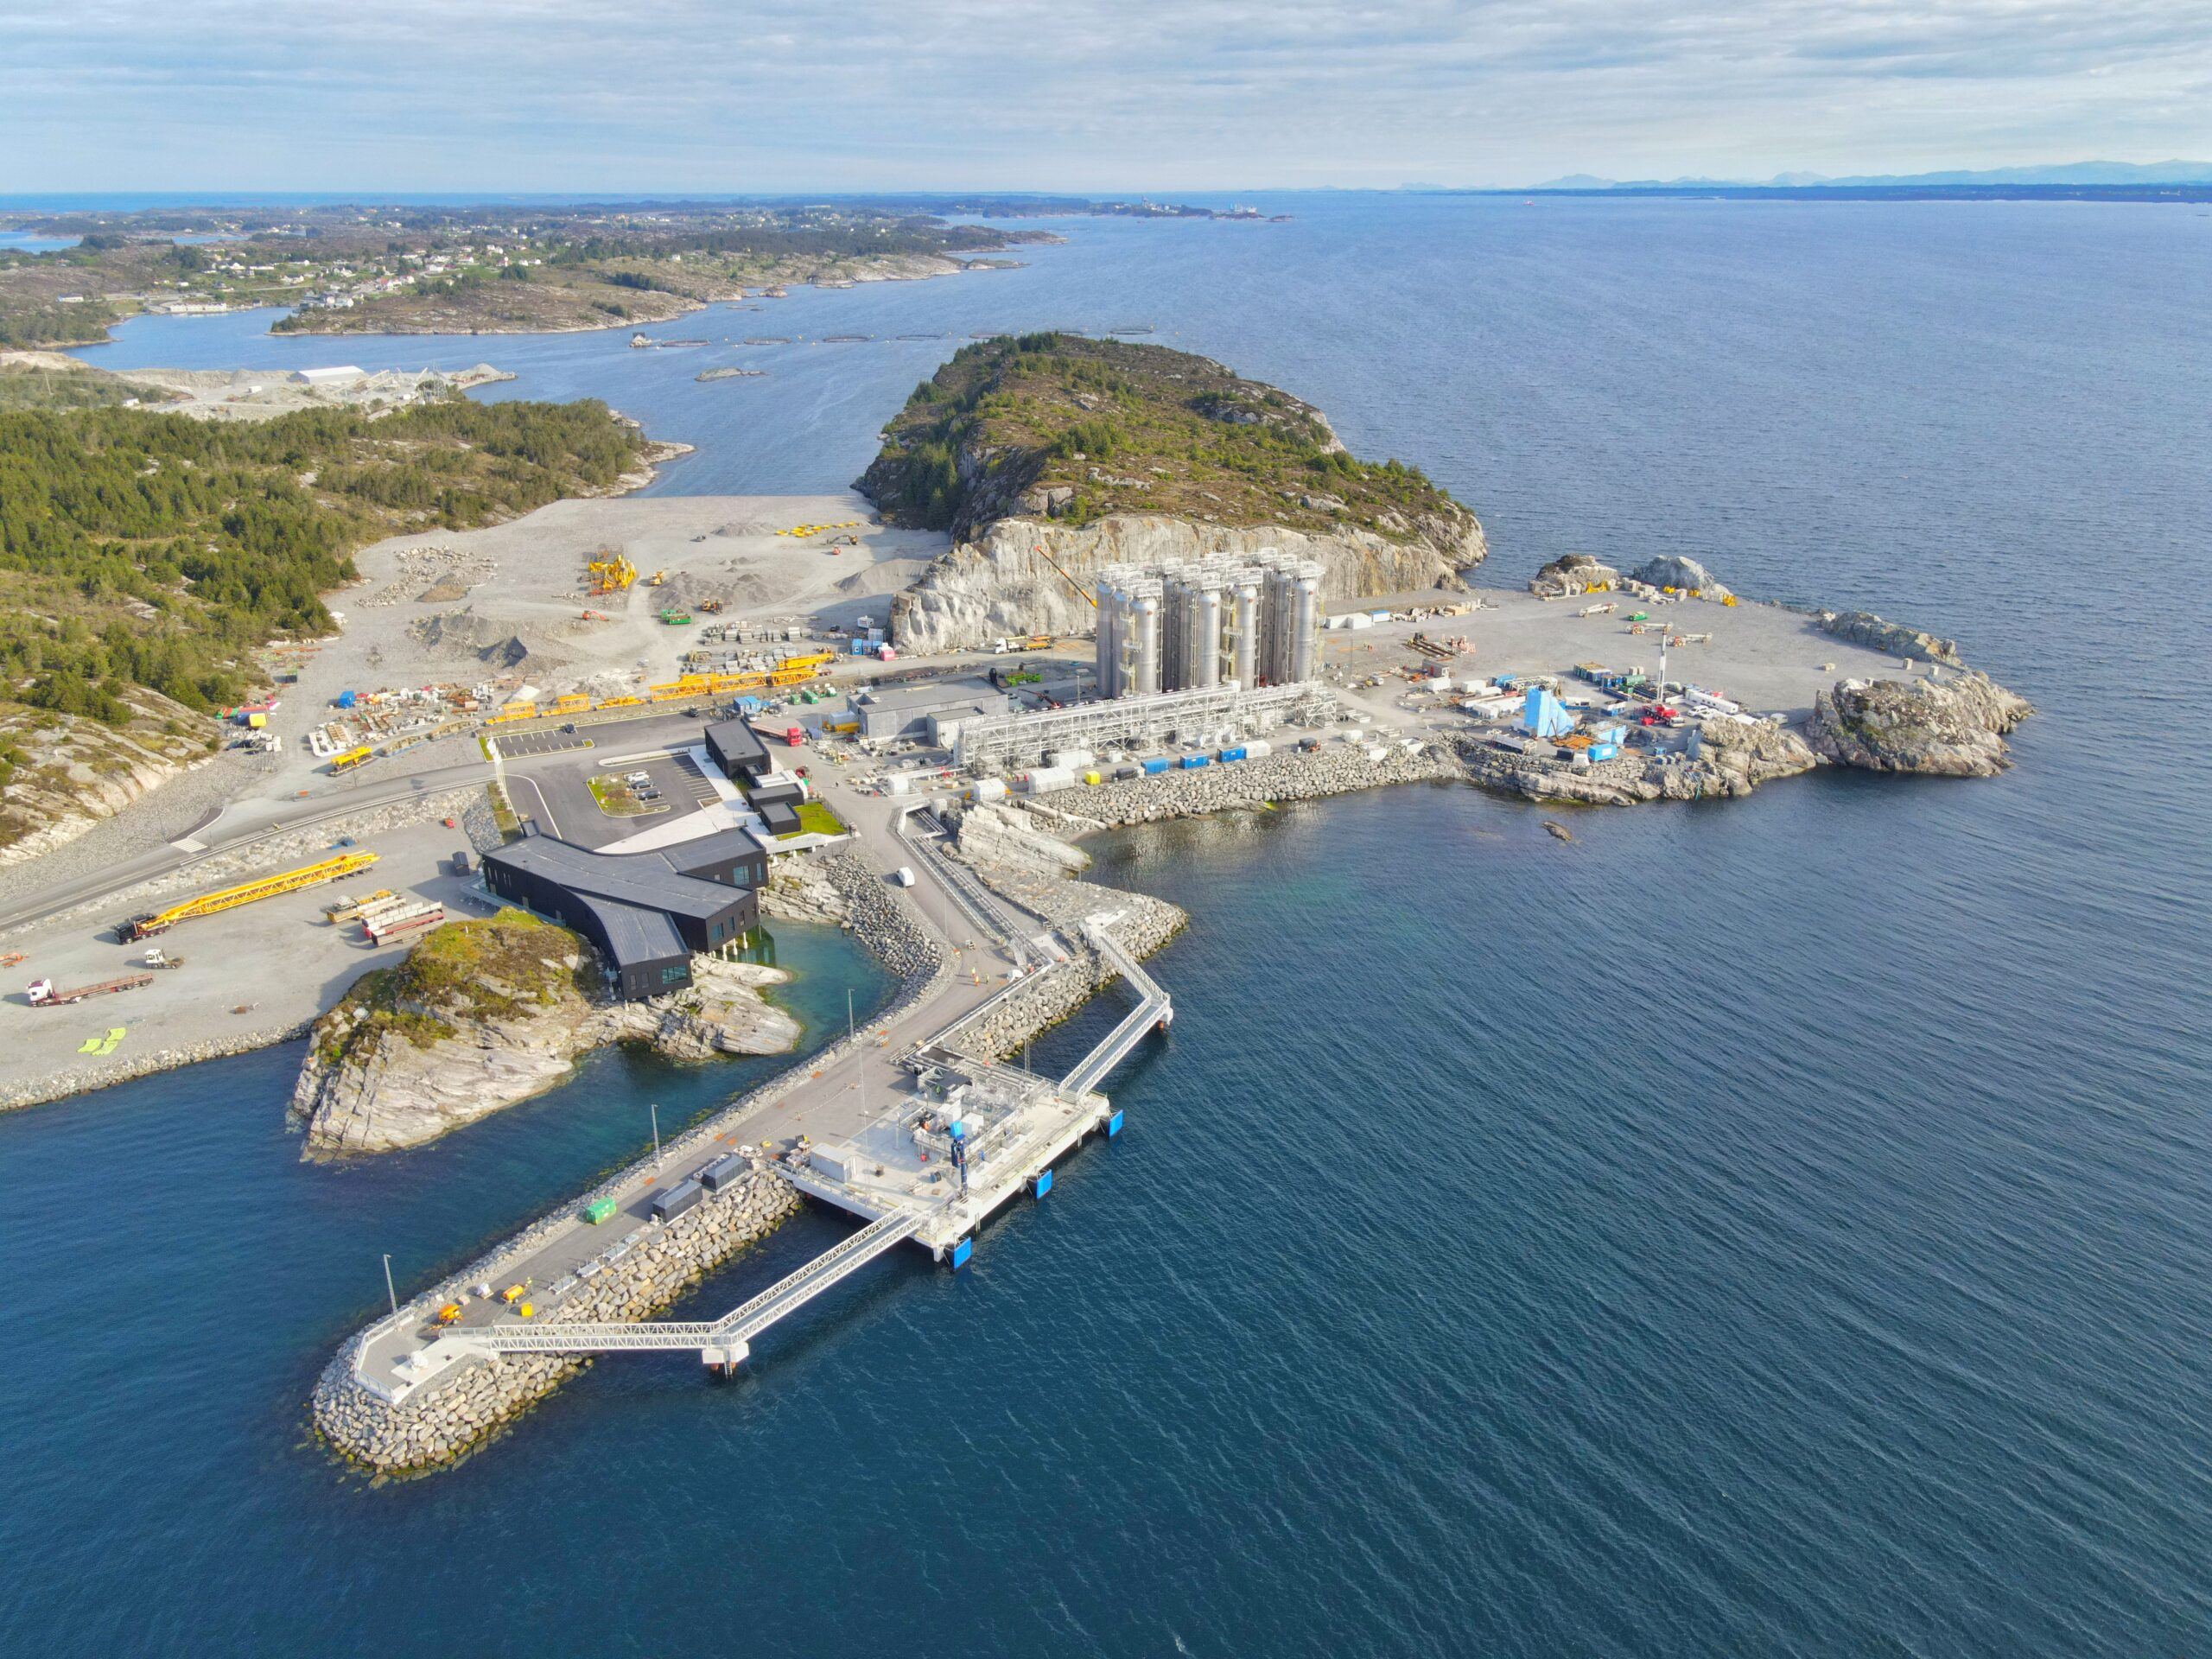
\includegraphics[width=0.6\textwidth, frame]{images/northern_lights.jpeg}
            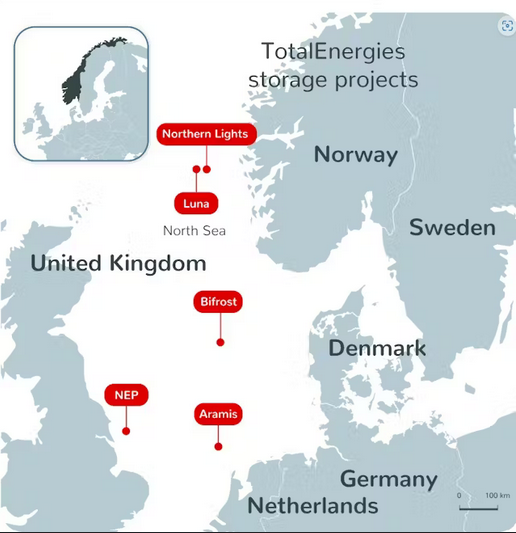
\includegraphics[width=0.6\textwidth, frame]{images/northern_lights_map.png}
        \end{figure}
    \end{column}
\end{columnframe}

\begin{frame}
    \begin{figure}
        \centering
        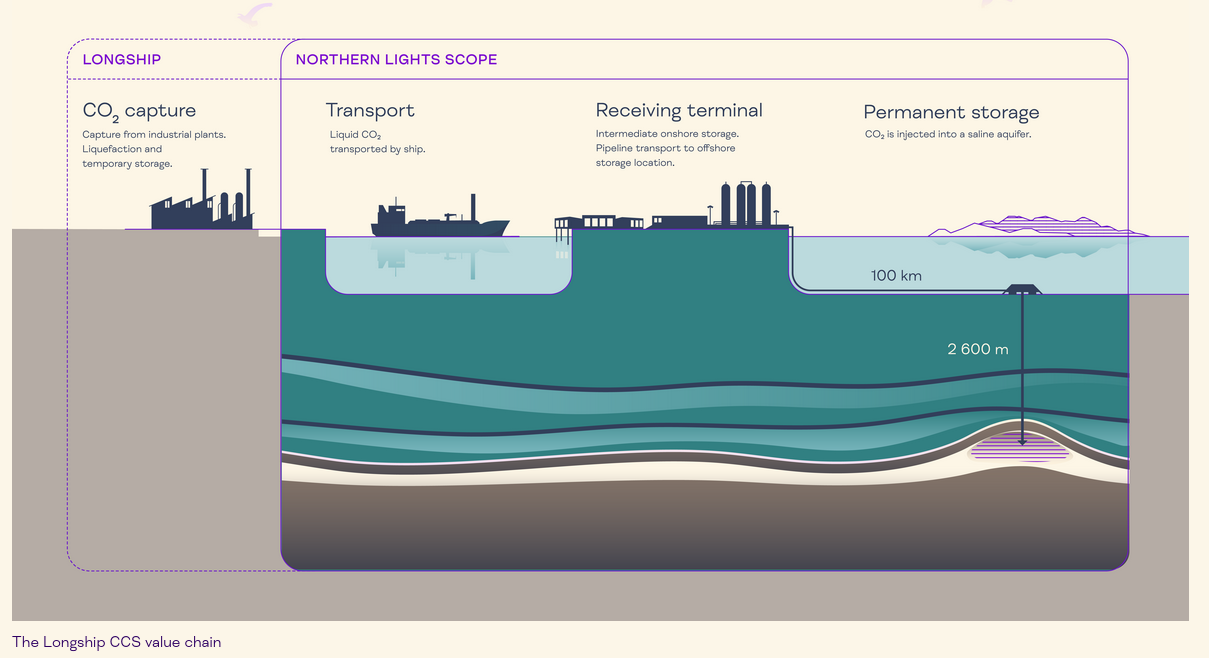
\includegraphics[width=1.0\textwidth, frame]{images/northern_lights_infographic.png}
    \end{figure}
\end{frame}

\begin{columnframe}{Studium przypadku: Orca (Hellisheidi, Islandia)}
    \begin{column}{0.5\textwidth}
        \begin{figure}
            \centering
            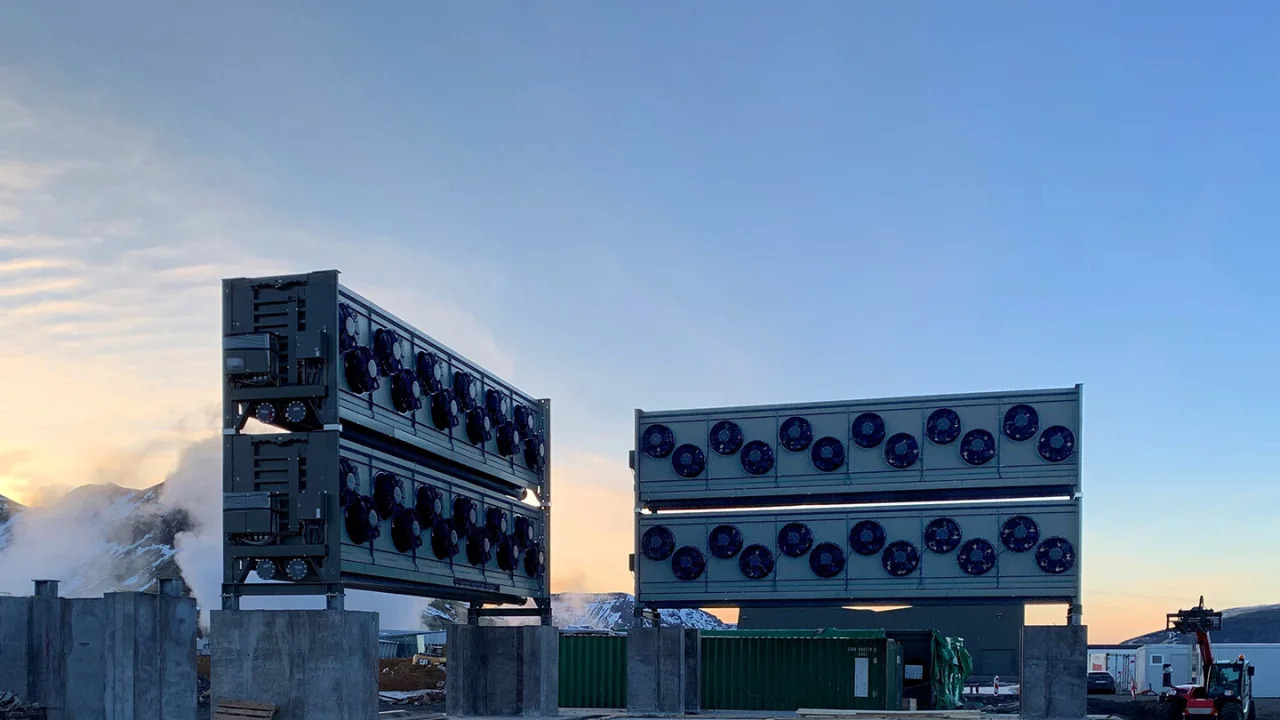
\includegraphics[width=0.9\textwidth, frame]{images/orca_iceland.jpg}
        \end{figure}
    \end{column}
    \begin{column}{0.5\textwidth}
        \begin{itemize}
            \item Wychwytywanie CO$_2$ z powietrza
            \item 500 (do 4000) ton CO$_2$ rocznie
        \end{itemize}
    \end{column}
\end{columnframe}

\begin{columnframe}{Studium przypadku: Mammoth (Islandia)}
    \begin{column}{0.5\textwidth}
        \begin{itemize}
            \item ok. 10x większa niż Orca
            \item budowa rozpoczęta w 2022 roku
            \item do 36 Mt CO$_2$ rocznie (!)
        \end{itemize}
    \end{column}
    \begin{column}{0.5\textwidth}
        \begin{figure}
            \centering
            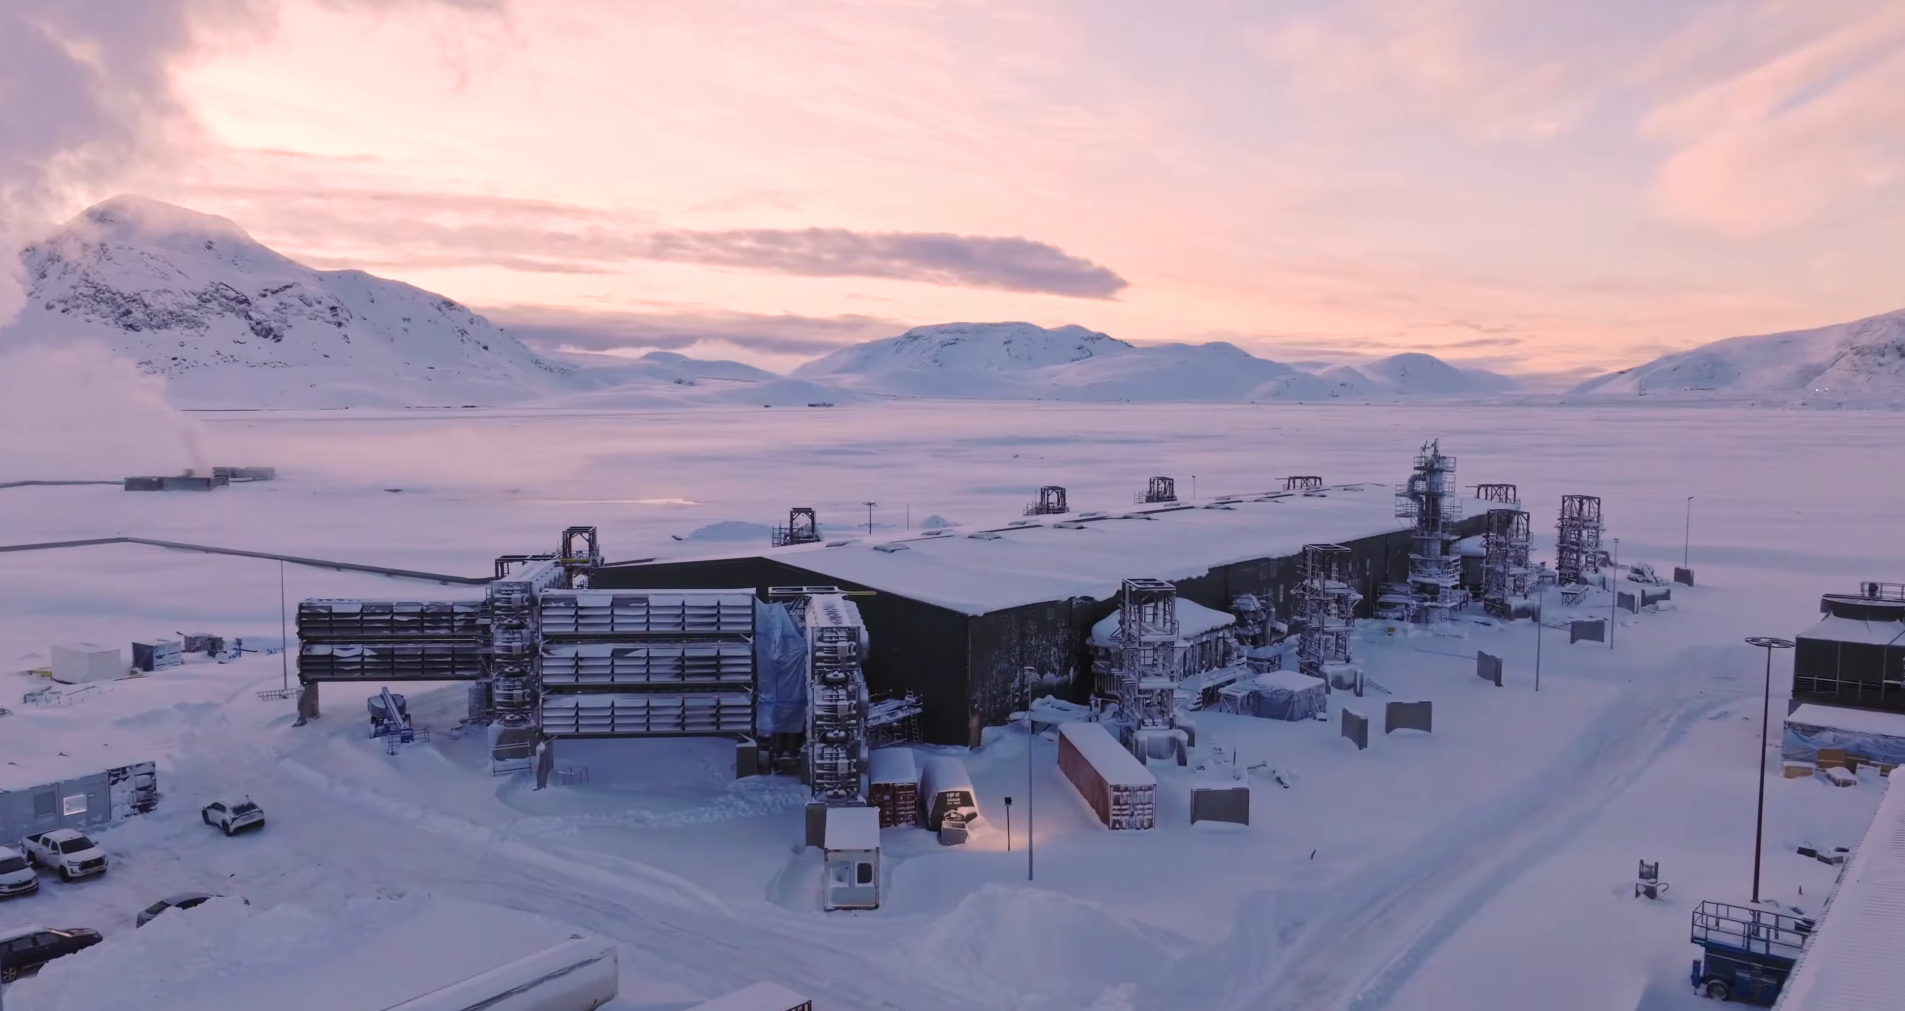
\includegraphics[width=0.9\textwidth, frame]{images/mammoth_iceland.png}
        \end{figure}
    \end{column}
\end{columnframe}

